%
% File eacl2017.tex
%
%% Based on the style files for ACL-2016
%% Based on the style files for ACL-2015, with some improvements
%%  taken from the NAACL-2016 style
%% Based on the style files for ACL-2014, which were, in turn,
%% Based on the style files for ACL-2013, which were, in turn,
%% Based on the style files for ACL-2012, which were, in turn,
%% based on the style files for ACL-2011, which were, in turn,
%% based on the style files for ACL-2010, which were, in turn,
%% based on the style files for ACL-IJCNLP-2009, which were, in turn,
%% based on the style files for EACL-2009 and IJCNLP-2008...

%% Based on the style files for EACL 2006 by
%%e.agirre@ehu.es or Sergi.Balari@uab.es
%% and that of ACL 08 by Joakim Nivre and Noah Smith

\documentclass[11pt]{article}

\usepackage[a4paper]{geometry}
\usepackage{eacl2017}
\usepackage{times}
\usepackage{url}
\usepackage{latexsym}

% Added from MacDonald's .tex file ----------------------------
\usepackage{float}
\usepackage{caption}

% amsmath package, useful for mathematical formulas
\usepackage{amsmath}

% amssymb package, useful for mathematical symbols
\usepackage{amssymb}

% hyperref package, useful for hyperlinks
% \usepackage{hyperref}

% graphicx package, useful for including eps and pdf graphics
% include graphics with the command \includegraphics
\usepackage{graphicx}

% Sweave(-like)
\usepackage{fancyvrb}
\DefineVerbatimEnvironment{Sinput}{Verbatim}{fontshape=sl}
\DefineVerbatimEnvironment{Soutput}{Verbatim}{}
\DefineVerbatimEnvironment{Scode}{Verbatim}{fontshape=sl}
\newenvironment{Schunk}{}{}
\DefineVerbatimEnvironment{Code}{Verbatim}{}
\DefineVerbatimEnvironment{CodeInput}{Verbatim}{fontshape=sl}
\DefineVerbatimEnvironment{CodeOutput}{Verbatim}{}
\newenvironment{CodeChunk}{}{}

% -------------------------------------------------------------------------

% Added so that I could use the `fancy_lists` pandoc extension. If you don't want this or it's giving you errors, remove the line below and the line in `acl_article.R` that adds `+fancy_lists`
\def\tightlist{}


\eaclfinalcopy
\def\eaclpaperid{}
% If you have:
%   final_submission: yes
%   eaclpaperid: <your ID number>
% in the .Rmd metadata, it should have automatically
% added "\eaclfinalcopy" and "\def\eaclpaperid{<your ID number>}" above


% You can expand the titlebox if you need extra space
% to show all the authors. You can do this by uncommenting
% the line in the Rmd header:
%   # titlebox_length: "5cm"
% and substituting it with your own length.
% Please note that the minimum length is 5cm--they will
% check it and make you change it if it's smaller than that.

\newcommand\BibTeX{B{\sc ib}\TeX}

\title{The Development of Abstract Concepts in Children's Early Lexical
Networks}


\author{{\large \bf Abdellah Fourtassi *}  \qquad {\large \bf Isaac L. Scheinfeld *} \qquad {\large \bf Michael C. Frank} \\ \texttt{\{afourtas, ischeinfeld, mcfrank\}@stanford.edu} \\ Department of Psychology \\ Stanford University}

\date{}

\begin{document}

\maketitle

\begin{abstract}
How do children learn abstract concepts such as animal vs.~artifact?
Previous research has suggested that such concepts can partly be derived
using cues from the language children hear around them. Following this
suggestion, we propose a model where we represent the children's
developing lexicon as an evolving network. The nodes of this network are
based on vocabulary knowledge as reported by parents, and the edges
between pairs of nodes are based on the probability of their
co-occurrence in a corpus of child-directed speech. We found that
several abstract categories can be identified as the dense regions in
such networks. In addition, our simulations suggest that these
categories develop simultaneously, rather than sequentially, thanks to
the children's word learning trajectory which favors the exploration of
the global conceptual space.
\end{abstract}

\section{Introduction:}\label{introduction}

One of the central challenges in cognitive development is to understand
how concepts develop \cite{carey2009,keil1992,gopnik1997}. Of particular
interest is the case of abstract concepts which have non-obvious shared
properties such as ``animal'' and ``artifact''. For example, a cat and a
bird are perceptually quite different but they share some fundamental
properties (e.g., breathing, feeding, and reproducing) which make them
animals (as opposed to artifacts). In such cases, learning requires in
part cultural/linguistic cues which provide information beyond what can
be obtained through the senses \cite{gelman2009,harris2012,csibra2009}.

One way children's conceptual learning can benefit from the language
they hear around them is through word co-occurrence. For example, one
can learn an abstract concept (e.g., animal) simply by observing how its
instances (e.g., ``cat'' and ``bird'') go together in speech. Indeed,
previous work has shown that the caregiver's input contains rich
co-occurrence information about various abstract concepts
\cite{huebner2018}. This work, however, has explored the conceptual
space from an adult perspective (using the words uttered by the
caregivers). Here we explore how abstract concepts may develop from the
children's perspective, investigating how their word learning trajectory
influences the higher-level organization of their developing lexicon.

We study the real conceptual development (i.e.~as induced by the real
trajectory of word learning) in comparison to two hypothetical
developmental scenarios induced by two divergent proposals about the
trajectory of word learning. On the first proposal, past lexical
knowledge facilitates the future learning of related words, e.g., the
word ``cat'' is more likely to be followed by another animal name than
it is to be followed by a food name \cite{steyvers2005,borovsky2016}. On
the second proposal, past lexical knowledge does not influence future
learning, e.g., learning the word ``cat'' does not necessarily increase
the odds that the next word will be another animal name
\cite{hills2009,sizemore2018}.

The paper is organized as follows. First, we describe the research
strategy. In brief, we represented the developing lexicon as an evolving
network and we used word co-occurrence in parent speech as a measure of
words' relatedness. We operationalized abstract concepts as the highly
interconnected regions of the network. Second, we explore how the
pattern of children's word learning influences higher-level conceptual
development, and whether this development corresponds to a simultaneous
or a sequential conceptual growth.

\begin{CodeChunk}
\captionsetup{width=0.8\textwidth}\begin{figure*}[h]

{\centering 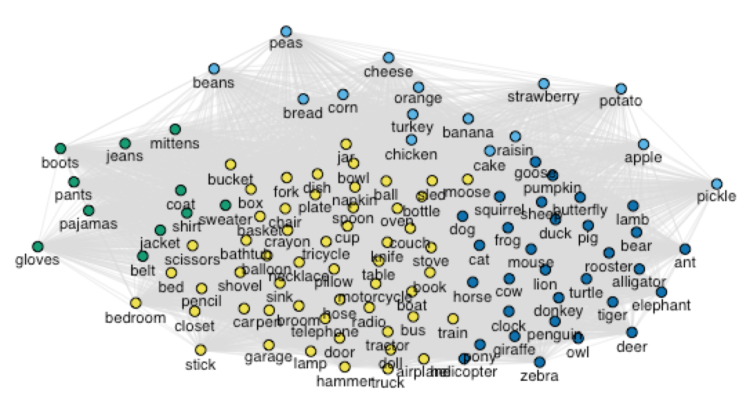
\includegraphics{figs/network-1} 

}

\caption[Network obtained using a sample of nouns in CDI data (nodes), and co-occurrence-based similarity from a corpus of child-directed speech (edges)]{Network obtained using a sample of nouns in CDI data (nodes), and co-occurrence-based similarity from a corpus of child-directed speech (edges). Colors indicate highly interconnected clusters identified using unsupervised network community detection. The clusters correspond, overall, to four higher-level concepts: animal, food, clothes, and artifacts.}\label{fig:network}
\end{figure*}
\end{CodeChunk}

\section{Data and Methods}\label{data-and-methods}

\subsection{Constructing Lexical
Networks}\label{constructing-lexical-networks}

The networks' nodes were nouns from Wordbank \cite{frank2017}, an open
repository aggregating cross-linguistic developmental data of the
MacArthur-Bates Communicative Development Inventory (CDI), a parent
report vocabulary checklist, Toddler version \cite{fenson94}. Pairs of
nouns were linked by weighted edges representing their semantic
similarity derived based on co-occurrence in the corpus of
child-directed speech CHILDES \cite{macwhinney2014}, using Word2Vec
algorithm \cite{mikolov2013}.

First, we constructed the end-state network based on all nouns learned
by the last age of acquisition. We used a subset of CDI nouns for which
cross-linguistic translations are present, allowing us to explore
cross-linguistic variability. We used data from the ten following
languages: Croatian, Danish, English, French, Italian, Norwegian,
Russian, Spanish, Swedish, and Turkish. The size of this subset varied
from 314 in Russian (representing 100\% of total nouns in this language)
to 176 in Turkish (representing 59.26\% of total nouns). Second, in
order to study development towards the end-state, we constructed a
different network at each month, based on the nouns that have been
learned by that month.

\subsection{Identifying Abstract Concepts in a
Network}\label{identifying-abstract-concepts-in-a-network}

We assume that abstract concepts correspond to clusters of highly
interconnected nodes in the networks. We identified such clusters using
WalkTrap \cite{pons2006}, an unsupervised community detection algorithm
based on the fact that a random walker tends to be trapped in dense
parts of a network. Figure \ref{fig:network} shows the outcome of
cluster identification in the end-state network in English. The
algorithm obtained four major clusters corresponding to the categories
of clothes, food, animal and artifacts. We refer to this end-state
clustering as \(\mathcal{C}^*\). To examine developmental change in the
conceptual organization, we ran the cluster identification algorithm at
each month of acquisition \(t\), and we compared the resulting
clustering, noted \(\mathcal{C}_t\), to that of the end-state
\(\mathcal{C}^*\). The method of this comparison is detailed below.

\begin{CodeChunk}
\captionsetup{width=0.8\textwidth}\begin{figure*}[h]

{\centering 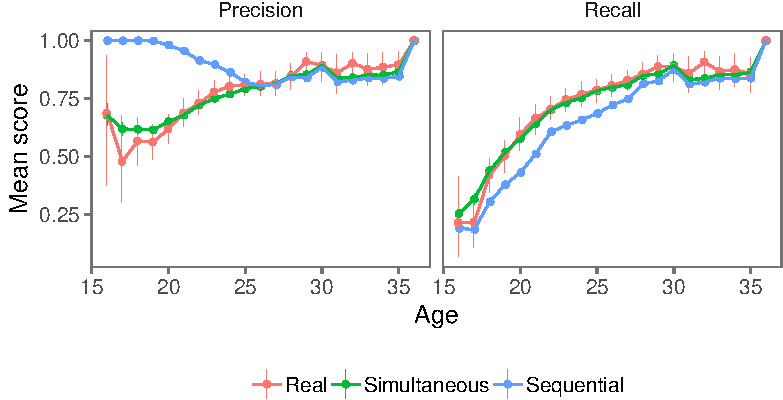
\includegraphics{figs/results-1} 

}

\caption[Mean precision and recall scores obtained through comparing the end-state clustering to clusterings at different months of acquisition, averaged across languages and numbers of clusters]{Mean precision and recall scores obtained through comparing the end-state clustering to clusterings at different months of acquisition, averaged across languages and numbers of clusters. Colors indicates real and hypothetical word sampling mechanisms. Errors bars represent 95\% confidence intervals.}\label{fig:results}
\end{figure*}
\end{CodeChunk}

\subsection{Measuring Conceptual
Development}\label{measuring-conceptual-development}

We measure conceptual development by comparing \(\mathcal{C}_t\) to
\(\mathcal{C}^*\) across time. We used a standard method in clustering
comparison, which is based on word pairs on which the two clusterings
agree or disagree \cite{rand1971,hubert1985}. We quantify clustering
comparison using precision \(P(\mathcal{C}_t)\) and recall
\(R(\mathcal{C}_t)\), defined as follows:

\[
P(\mathcal{C}_t) = \frac{|tp(\mathcal{C}_t)|}{|tp(\mathcal{C}_t)| + |fp(\mathcal{C}_t)|}
\]

\[
R(\mathcal{C}_t) = \frac{|tp(\mathcal{C}_t)|}{|tp(\mathcal{C}_t)| + |fn(\mathcal{C}_t)|}
\] Where \(tp(\mathcal{C}_t)\) are the true positives, defined as the
word pairs that are placed in the same cluster under \(\mathcal{C}_t\)
and in the same cluster under \(\mathcal{C}^*\). \(fp(\mathcal{C}_t)\)
are the false positives defined as the pairs placed in the same cluster
under \(\mathcal{C}_t\) and in different clusters under
\(\mathcal{C}^*\). Finally, \(fn(\mathcal{C}_t)\) are the false
negatives defined as the pairs placed in different clusters under
\(\mathcal{C}_t\) and in the same cluster under \(\mathcal{C}^*\).

We made this comparison using different degrees of clustering
granularity. More precisely, we fixed the same number of clusters for
\emph{both} \(\mathcal{C}_t\) and \(\mathcal{C}^*\), and we varied this
number from two to four clusters. We did not use the trivial case of one
cluster, nor did we use more than four clusters, since this number was
optimal for the largest network (i.e., the end-state network) based on
the modularity maximization criterion \cite{newman2006}.

\subsection{Learning Mechanisms}\label{learning-mechanisms}

We examined how abstract concepts develop under an average word learning
trajectory derived from real developmental data. To construct this
trajectory, we used the normative age of acquisition, that is, the age
at which a word is produced by at least 50\% of children in each
language \cite{goodman2008}. As mentioned above, we compared this
development to the development induced by a first hypothetical
trajectory where known words influence future word learning and a second
hypothetical trajectory where learning proceeds regardless of what words
are already known.

We instantiated the first trajectory through sampling from one
conceptual category at a time: the first word is selected randomly from
one cluster, subsequent words are sampled from the same cluster. After
all words from this cluster are used, a word from a different cluster is
chosen, and the same process is repeated until all clusters are covered.
We call this sampling procedure the \emph{sequential model}. We
instantiated the second trajectory through a uniform sampling across
time from the end-state vocabulary. We call this sampling procedure the
\emph{simultaneous model}.

\section{Results}\label{results}

Figure \ref{fig:results} shows the scores obtained through comparing
\(\mathcal{C}^*\) to \(\mathcal{C}_t\) at different points in time
\(t\). For the real word learning trajectory, both precision and recall
start relatively low, indicating that the induced conceptual
organization is initially quite different from that of the end-state.
Both measures converge towards 1 (i.e., perfect score) as
\(\mathcal{C}_t\) becomes more and more similar to \(\mathcal{C}^*\).

The simultaneous model mimics closely the patterns of real conceptual
development, explaining almost all the variance in mean precision
(\(R^2 =\) 0.94) and recall (\(R^2 =\) 0.99). In contrast, the
sequential model had generally a higher precision, i.e., it induced
fewer false positive pairs. This result is due to the fact that we
sampled instances from the same category. However, the same model had
generally lower recall scores, i.e., it induced more false negative
pairs. This second result was due to the fact that sampling from the
same category leads to clusterings that are finer in their conceptual
granularity than the end-state. As a consequence of this discrepancy
with respect to real development, the sequential model explained less
variance than the simultaneous model did in both its mean precision
(\(R^2 =\) 0.44) and recall (\(R^2 =\) 0.96).

\section{Discussion}\label{discussion}

Can children learn abstract concepts based on word co-occurrence in the
language they hear around them? Previous work has shown that
child-directed speech contains information about several abstract
concepts \cite{huebner2018}. Here we investigated when and how this
information becomes available to children as their lexical network
grows. We found that even with a small lexicon, several high-level
concepts such as ``animal'', ``artifact'', ``food'' and ``clothes''
emerge bottom-up as clusters of highly interconnected nodes in the
network. Furthermore, compared with a model that posited sequential
learning, we found that these categories tended to emerge in concert
with one another.

The development of the higher-level conceptual structure seems to be
unaffected by the order with which words are acquired (as long as this
order approximates a uniform sampling from the end-state lexicon),
suggesting that the process of conceptual development can accommodate a
wide range of word learning trajectories without a qualitative change in
the higher-level organization. For example, whether acquisition starts
first with the words ``cat'' and ``banana'' or with the words ``cow''
and ``potato'' does not qualitatively affect the higher-level
organization involving ``animal'' and ``food''. This property is
important as it suggests, for instance, that development is resilient to
variability in the children's linguistic input
\cite{slobin2014,hart1995}.

Developmental changes were captured by precision and recall. The
increase in precision means that false positives decrease over time:
some word pairs that are initially lumped together in a same category,
are eventually differentiated. Similarly, the increase in recall means
that false negatives decrease, that is, some word pairs that are
initially distinct, become eventually subsumed by a same category. These
patterns suggest a process of conceptual reorganization involving both
``differentiation'' and ``coalescence'' as has been suggested in the
developmental literature \cite{carey2009}.

That said, these developmental changes were not necessarily related to
specific concepts (since the patterns were similar in the simultaneous
model where we randomized the order of word learning). Instead, this
finding suggests that differentiation and coalescence of word pairs in
our data are related to the change in the vocabulary size across
development: As more words are added to their lexical network, learners
may approximate better the underlying conceptual organization of the
mature lexicon and would make fewer categorization errors. Indeed,
research in network science indicates that properties of a real network
become more distorted as the size of a sampled sub-network decreases
\cite{leskovec2006}.

One limitation of this study is that we used the normative age of
acquisition, computed using different children at different age groups.
This choice was due to the cross-sectional nature of available CDI data.
Though such a measure has been widely used to study important aspects of
the early lexical networks \cite{hills2009,stella2017,storkel2009}, it
only applies at the population level. In our case, though we found that
concepts develop simultaneously, individual children may display, at
least locally, a sequential-like behavior. For example, prior knowledge
about dinosaurs may enable the learning of new dinosaur-related words
more easily \cite{chi1983}.

In sum, this work provided a quantitative account of how abstract
concepts can emerge from the interaction of the children's emerging
vocabulary and the properties of their linguistic input. One important
direction for future work is to investigate the extent to which the
correlational findings obtained in this study (e.g., the identity of
categories formed across development or the fact that categorization
errors decrease with the size of the lexicon) can be corroborated by
controlled behavioral experiments.

\vspace{1em}

\fbox{\parbox[b][][c]{7.3cm}{\centering All data and code are available at https://github.com/afourtassi/conceptNet}}
\vspace{1em}

\bibliography{eacl2017}
\bibliographystyle{eacl2017}

\end{document}

